\section{Regenerated demonstrator results}
\label{sec:results}
\subsection{Scenario design and performance measures}
All reported results are synthetic and were regenerated after the scientific revision. The shared seed is 20260908. A model year is 365.25 days. The baseline uses a 10~mm core with 4~kg\,m$^{-2}$ dry loading, nine tiles and complete geometric coverage of the hypothetical hotspot. Scenario F changes both geometry and transport and is therefore a compound stress case.

\begin{table}[htbp]\centering\small
\caption{Configured six-scenario experiments.}\label{tab:scenarios}
\begin{tabular}{llrp{.48\linewidth}}\toprule
ID & Scenario & Years & Change \\
\midrule
A & Fresh mat & 1 & Baseline source and fresh medium. \\
B & Progressive loading & 6 & Same physical configuration, longer exposure. \\
C & Increased source & 6 & At year 2, porewater concentrations triple and seepage doubles. \\
D & Local damage & 4 & Displacement at year 1.5; another tile loses 35\% integrity at year 2.2. \\
E & Delayed chemistry & 4 & 75-day lab delay, probe dropout at years 1--1.25 and subsequent drift. \\
F & Undersized mat & 4 & 45\% footprint, four tiles, 2~mm core, 10\% edge bypass and tripled seepage. \\
\bottomrule\end{tabular}\end{table}

The principal attenuation is the whole-hotspot quantity
\begin{equation}
A_{\mathrm{area},e}(t)=1-\frac{\int_{\Omega_h}J_{\mathrm{res},e}(x,y,t)\,\mathrm{d}A}{|\Omega_h|J_{\mathrm{bare},e}(t)}.
\end{equation}
It includes uncovered area, physical damage and bypass. The raw-column attenuation remains a separate diagnostic. The barrier-only comparator applies the same area weighting to the exact stationary discrete column with uptake disabled. Its difference from transient total attenuation is a diagnostic increment, not an isolated measurement of chemistry: transient porewater storage also contributes.

The endpoint concentration ratio is $R_{\max,e}=\max c_{\mathrm{with},e}/\max c_{\mathrm{bare},e}$. Its two maxima need not occur in the same cell. Neither source attenuation nor this ratio is a toxicity or compliance metric. Retained column mass comprises porewater and sorbed inventory; the active and retrieved parts are recorded separately.

\subsection{Final states and chemical contribution}
\begin{table}[htbp]\centering\small
\caption{Final whole-hotspot attenuation and nominal sorbed-capacity use (percent). No statistical confidence interval is implied.}\label{tab:all-metals}
\begin{tabular}{lrrrrrr}\toprule
Scenario & $A_{\rm Pb}$ & $A_{\rm Hg}$ & $A_{\rm Cu}$ & $q_{\rm Pb}/q_{\max}$ & $q_{\rm Hg}/q_{\max}$ & $q_{\rm Cu}/q_{\max}$ \\
\midrule
A & 89.93 & 91.92 & 87.13 & 44.69 & 0.36 & 8.70 \\
B & 61.32 & 61.57 & 61.19 & 66.76 & 0.83 & 9.53 \\
C & 57.91 & 58.09 & 57.92 & 100.00 & 2.75 & 30.62 \\
D & 70.21 & 70.99 & 69.99 & 63.31 & 0.74 & 9.11 \\
E & 71.75 & 72.40 & 71.59 & 64.01 & 0.76 & 9.15 \\
F & 25.87 & 25.87 & 25.85 & 66.60 & 0.85 & 9.41 \\
\bottomrule\end{tabular}\end{table}

\begin{table}[htbp]\centering\small
\caption{Final footprint after physical condition, Pb column inventories and monitoring workload. Coverage excludes edge/fouling bypass; records include explicit missing results.}\label{tab:scenario-results}
\begin{tabular}{lrrrrr}\toprule
Scenario & Coverage (\%) & Active Pb (kg) & Retrieved Pb (kg) & Services & Records \\
\midrule
A & 100.00 & 6.884 & 0 & 0 & 4950 \\
B & 100.00 & 10.28 & 0 & 0 & 29349 \\
C & 100.00 & 15.45 & 0 & 0 & 29349 \\
D & 96.11 & 9.752 & 0.9153 & 1 & 19593 \\
E & 100.00 & 9.859 & 0 & 0 & 19593 \\
F & 45.00 & 0.9233 & 0 & 0 & 11995 \\
\bottomrule\end{tabular}\end{table}

Increasing occupancy does not imply full exhaustion. A low accessible concentration or partition slope can hold the equilibrium load below the allocated capacity. Conversely, decreasing effective coverage can worsen hotspot emission even if surviving columns remain effective. The scenario-D time series now resolves the local physical events at their true times. Any accepted service changes active-media inventory and restores the serviced tile's condition; retrieved mass remains in its separate ledger.

\begin{table}[htbp]\centering\small
\caption{Resolved Pb jumps at a shared event time. The flux ratio is immediately after divided by immediately before; attenuation can rise while absolute emission rises because its bare-source denominator also changes.}\label{tab:event-jumps}
\begin{tabular}{llrrrr}\toprule
ID & Event & Age (yr) & Before (\%) & After (\%) & Flux ratio \\
\midrule
C & Source increase & 2 & 82.72 & 85.08 & 2.737 \\
D & Displacement & 1.5 & 85.99 & 76.44 & 1.682 \\
D & Replacement & 2.053 & 73.24 & 84.13 & 0.593 \\
D & Integrity loss & 2.2 & 83.27 & 80.10 & 1.189 \\
\bottomrule\end{tabular}\end{table}

In scenario C, the source step raises the absolute residual flux even though the instantaneous attenuation ratio improves. Subsequent storage adjustment and Pb capacity locking explain the later bend. In D, the upward jump follows the recorded replacement of a displaced tile; it is followed by a separate integrity-loss event on another tile. These events are explicit changes in the model state, not measurement noise.

\figpage{attenuation_all}{Whole-hotspot attenuation in all six regenerated scenarios. The shared axis includes the complete response of the undersized design. Event-time discontinuities are retained rather than smoothed.}{fig:attenuation}
\figpage{saturation_all}{Sorbed inventory as a fraction of allocated nominal capacity. The profiles are deterministic simulations; low capacity use can coexist with little incremental uptake.}{fig:saturation}
\figpage{condition_all}{Mean fouling, physical integrity and actual hotspot coverage through time. Matching physical histories overlap. Coverage and bypass are distinct: a nominally intact footprint can still lose effective performance as fouling diverts flow.}{fig:condition}
\begin{table}[htbp]\centering\small
\caption{Six-year baseline decomposition using a common discrete transport operator and hotspot weighting. Differences are percentage points.}\label{tab:barrier}
\begin{tabular}{lrrr}\toprule
Element & Total (\%) & Barrier reference (\%) & Difference (pp) \\
\midrule
Pb & 61.32 & 61.19 & 0.1279 \\
Hg & 61.57 & 61.19 & 0.3759 \\
Cu & 61.19 & 61.19 & 0.005172 \\
\bottomrule\end{tabular}\end{table}

The baseline chemical increment is much smaller than the total attenuation. Cumulative storage and an endpoint increment answer different questions: mass retained during an earlier uptake transient can remain in the core even when the later flux approaches a resistance-controlled regime. Subtracting an approximate continuum barrier from a discrete transient result previously introduced small misleading differences, especially for Cu; the revised reference removes that operator mismatch.

\subsection{Spatial source and water transport}
All standard plume windows last 24 hours. The comparison below uses a three-year mat state when that age is within the scenario horizon, and the actual one-year endpoint for A. The source is held fixed during each window and the water starts clean. The final-age source plate in Appendix~\ref{app:spatial} additionally shows each scenario endpoint.
\begin{table}[htbp]\centering\small
\caption{Pb comparison at the stated mat age. Source is kg per 24-hour window; endpoint concentration maxima are ng/L.}\label{tab:spatial-results}
\begin{tabular}{lrrrrrrr}\toprule
ID & Age (yr) & Bare kg & Mat kg & Reduction (\%) & Bare peak & Mat peak & $R_{\max}$ \\
\midrule
A & 1 & 0.2931 & 0.0295 & 89.93 & 59.99 & 6.039 & 0.1007 \\
B & 3 & 0.2931 & 0.06726 & 77.05 & 39.37 & 9.035 & 0.2295 \\
C & 3 & 0.929 & 0.2535 & 72.71 & 124.8 & 34.06 & 0.2729 \\
D & 3 & 0.2931 & 0.07169 & 75.54 & 39.37 & 10.32 & 0.2621 \\
E & 3 & 0.2931 & 0.06726 & 77.05 & 39.37 & 9.035 & 0.2295 \\
F & 3 & 0.3262 & 0.2351 & 27.95 & 43.83 & 28.29 & 0.6454 \\
\bottomrule\end{tabular}\end{table}

Unlike the previous geometry, the configured damaged tiles intersect the hotspot. Their source changes are therefore represented spatially. Scenario E changes observation timing rather than material coefficients; equality with a matched physical trajectory is expected whenever the policy produces the same servicing history. Scenario F leaves 55\% of the hotspot geometrically uncovered before bypass, so its column performance cannot be presented as whole-area performance.

\figpage{flux_30}{Regenerated residual Pb source maps at three years, or the actual one-year endpoint for A, with one shared source scale. Ages are shown in each panel.}{fig:fluxlate}
\figpage{spatial_B}{Baseline B at three years: matched with/without endpoint water concentrations, their cellwise ratio, and effective reactive cover.}{fig:spatialB}
\figpage{profiles_all}{Final Pb profiles through the core for every scenario. Colours show local sorbed load in mg per kg of core; panel scales are stated separately. Similar tiles are deterministic columns, not independent experimental replicates.}{fig:profiles}
\begin{figure}[htbp]\centering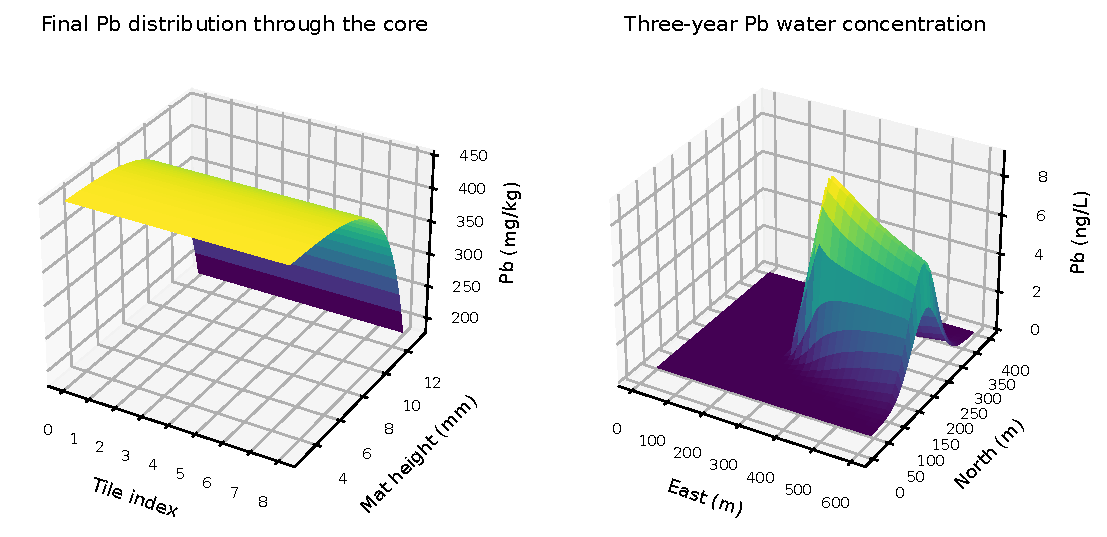
\includegraphics[width=\linewidth]{figures/surfaces.pdf}
\caption{Final six-year baseline Pb load through the core and the three-year endpoint plume shown as surfaces. Height denotes different labelled quantities; concentration is not seabed elevation.}\label{fig:surfaces}\end{figure}

\subsection{Three maintenance policies on a common emission basis}
The comparison uses identical source and forcing assumptions, seed and nominal monitoring configuration. Calendar and evidence-informed servicing share the actual sample calendar; the bare reference has no installed-mat observations. All policies integrate the same whole-hotspot residual source, including uncovered and bypassed area. Calendar service is triggered on the next decision boundary after its interval is reached; the baseline services occur on days 750 and 1500. Evidence-informed service depends on arrived compatible measurements, their quality, attribution and uncertainty. The economic column below is the assumed service ledger; it excludes full lifecycle costs.
\begin{table}[htbp]\centering\small
\caption{Six-year cumulative whole-hotspot emission (kg), service events and assumed service expenditure.}\label{tab:policies}
\begin{tabular}{lrrrrr}\toprule
Policy & Pb emitted & Hg emitted & Cu emitted & Services & Cost (EUR) \\
\midrule
No mat & 642.3 & 5.138 & 1285 & 0 & 0 \\
Calendar & 62.74 & 0.4271 & 163.8 & 2 & 3.734e+06 \\
Evidence & 141.6 & 1.08 & 297.9 & 0 & 0 \\
\bottomrule\end{tabular}\end{table}

\begin{table}[htbp]\centering\small
\caption{Pb inventory accounting in the policy comparison. Column inputs and outputs use the full tile-column control volume and are not added to the area-mixed emission above.}\label{tab:policy-ledger}
\begin{tabular}{lrrrr}\toprule
Policy & Column input (kg) & Active (kg) & Retrieved (kg) & Column out (kg) \\
\midrule
No mat & 0 & 0 & 0 & 0 \\
Calendar & 42.77 & 8.832 & 18 & 15.94 \\
Evidence & 38.71 & 10.28 & 0 & 28.43 \\
\bottomrule\end{tabular}\end{table}

\figpage{policy}{Policy comparison using whole-hotspot Pb emission for every policy. Active plus retrieved column inventory is shown separately. Costs are assumed service expenditure, not total project cost or profit.}{fig:policy}
Sparse Pb/Hg chemistry constrains evidence-informed decisions. Cu is simulated but not observed, and missing Cu no longer contributes evidence of performance loss. Unknown source and flux intervals are identified explicitly; no interval midpoint is a field measurement. Recommendations to sample or inspect do not adapt the future campaign schedule in this demonstrator. This comparison therefore does not establish the value of an optimised monitoring programme.

\subsection{Integration and conservation checks}
The regenerated audit compares final timeline flux with the integrated spatial source for every element and policy, validates every plume age against its simulation horizon, checks observation-ID uniqueness, and checks all individual column and water ledgers. Initial samples are unadvanced; the integration ends at the exact requested time, including a partial last step. The zero-sorption reference is tested against independent stationary face balances and grid refinement, and nonlinear transient profiles against an adaptive ODE reference.
\begin{table}[htbp]\centering\small
\caption{Audit of regenerated scenario outputs. Relative errors are dimensionless. Conservation and agreement are numerical checks, not material validation.}\label{tab:scenario-audit}
\begin{tabular}{lrrll}\toprule
ID & Worst budget error & Source agreement error & Valid ages & Unique IDs \\
\midrule
A & 3.371e-14 & 9.245e-15 & True & True \\
B & 1.661e-13 & 2.062e-15 & True & True \\
C & 1.439e-13 & 1.872e-15 & True & True \\
D & 9.371e-14 & 2.496e-15 & True & True \\
E & 1.101e-13 & 2.637e-15 & True & True \\
F & 5.685e-14 & 3.026e-16 & True & True \\
\bottomrule\end{tabular}\end{table}

% Generated by tools/render_numerical_results.py; values come from audit JSON.
\subsection{Independent numerical verification and discontinuities}
\label{sec:numerical_revision}

The revised code was checked against independently assembled stationary
face balances, a continuum transport solution and adaptive backward
differentiation formula (BDF) integration of the coupled semi-discrete
transport--sorption equations. These checks address equation solving and
discretisation separately from a mass ledger. The complete integrated test
suite is reported separately; the focused checks below address independent
oracles, source discontinuities and exact reuse of equivalent tile states.

For a short nonlinear test, the reference column was set to eight cells and
capacity $10^{-5}$~kg/kg, so that breakthrough occurs within fourteen days.
This is an accelerated verification problem, not a revised material
calibration. Concentration and sorbed-profile errors were normalised by
$10^{-3}$~kg/m$^3$ and capacity, respectively, and compared at daily marks.
The reference uses SciPy~1.18.1's variable-order BDF integration with relative
tolerance $2\times10^{-9}$ and absolute tolerance $10^{-14}$.\citep{scipy_solve_ivp}
Table~\ref{tab:independent-temporal} reports the maximum normalised
profile error, not a fitted coefficient or an assumed precision.


\begin{table}[htbp]\centering\small
\caption{Convergence of the nonlinear column to independent adaptive BDF integration in the accelerated verification problem.}\label{tab:independent-temporal}
\begin{tabular}{rr}\toprule
Step (h) & Maximum normalised profile error \\\midrule
6 & 0.0947294 \\
3 & 0.0534873 \\
1.5 & 0.03128 \\
\bottomrule\end{tabular}\end{table}


\begin{table}[htbp]\centering\small
\caption{Spatial refinement of the non-sorbing reference column against its continuum solution. The approximately halving error is consistent with first-order upwind transport.}\label{tab:independent-spatial}
\begin{tabular}{rr}\toprule
Layer cells & Relative stationary flux error (\%) \\\midrule
20 & 1.12686 \\
40 & 0.564771 \\
80 & 0.2825 \\
160 & 0.141248 \\
\bottomrule\end{tabular}\end{table}


The largest per-step mass residual in this nonlinear verification was $1.60308\times10^{-20}$~kg/m$^2$, with zero recorded clipping. The finite temporal errors in Table~\ref{tab:independent-temporal} show why conservation cannot establish accuracy. The runtime now refuses unconverged sorption branch masks with an instruction to reduce the step or increase the iteration limit.


Within-call reuse of exactly equivalent vertical tile states was also checked against independent per-tile advancement. Fourteen additional regression cases preserve complete step results, identities and independent arrays. A 30-day full-history comparison was bitwise identical across all result fields. One exploratory timing gave 2.14-fold speedup; the recorded repeat under concurrent workload gave 1.17-fold (6.62 versus 7.75~s). Runtime depends on workload; nine equivalent solver calls being reduced to one does not imply ninefold end-to-end acceleration. The benchmark artifact and reproduction script accompany the repository.


The exact discrete barrier also removes a mismatch in the former diagnostic:
the old continuum approximation double-counted a top half-cell resistance and
approximated advective bottom resistance. At the default clean state, the
corrected barrier flux is 2.1346\% higher for Pb and Hg and 2.7534\% higher for
Cu than that old comparison. This changes the interpretation of the plotted
barrier; it does not alter the transport trajectory or calibrate the material.

Two remaining types of abrupt behaviour have explicit causes. First, a step
in the prescribed source changes the denominator of
$1-J_{\mathrm{out}}/J_{\mathrm{bare}}$ immediately, whereas porewater storage
is continuous. A tenfold source decrease produces a tenfold instantaneous
increase in that residual ratio, followed by washout
(Figure~\ref{fig:reactive-numerical-audit}D). Such a ratio dip is compatible
with a conserving solver. Second, the capacity-lock law itself is
discontinuous: an exactly full cell is held, but a cell just below capacity
can desorb. In a six-hour, one-cell clean-water flush, an exactly full state
gives zero outgoing flux; starting at $q/Q=1-10^{-10}$ gives
$9.8426\times10^{-12}$~kg/m$^2$/s. This is an unvalidated constitutive
assumption retained explicitly, not evidence that real keratin exhibits that
switch. No plotted trajectory was smoothed to conceal these effects.


\begin{figure}[htbp]\centering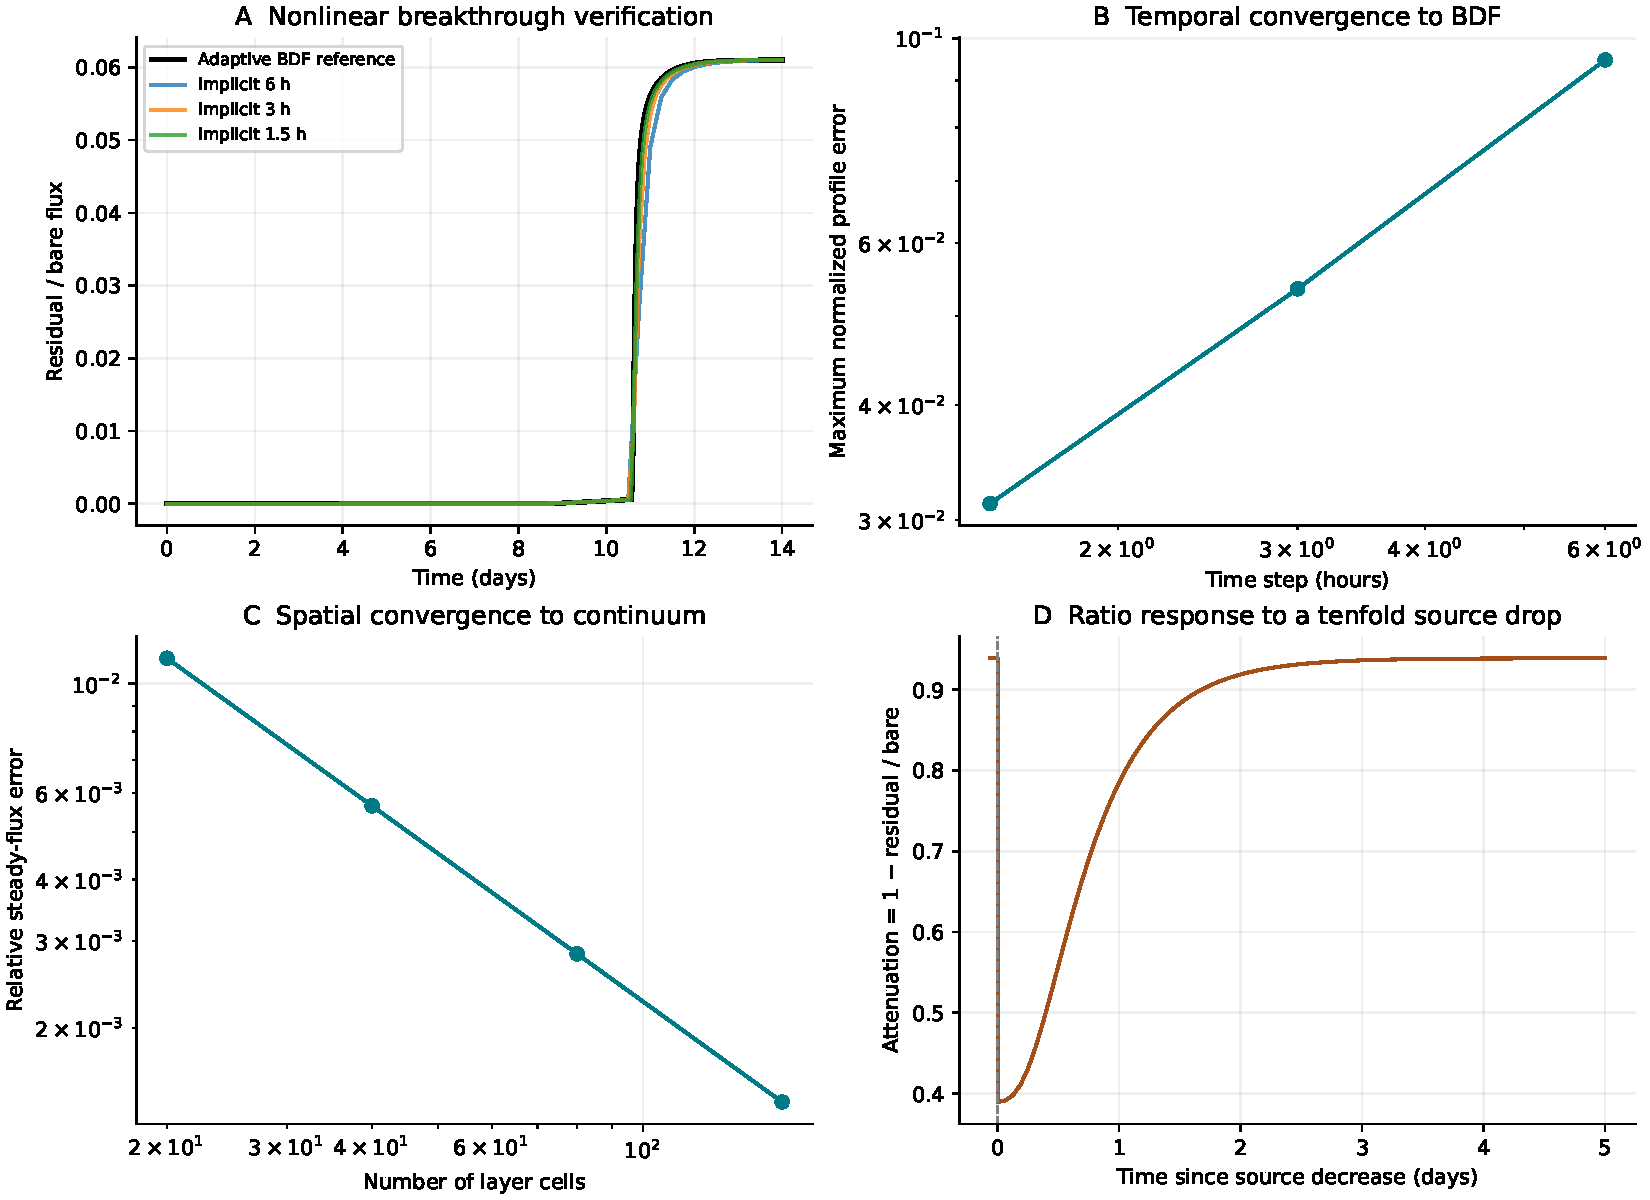
\includegraphics[width=\linewidth]{figures/reactive_numerical_audit.pdf}
\caption{Independent column verification and a forcing-induced ratio dip. A: nonlinear breakthrough against adaptive BDF; B: the maximum normalised profile error under time refinement; C: stationary flux error under spatial refinement; D: instantaneous ratio change and subsequent washout after a tenfold source decrease. The low-capacity test in A--B accelerates verification and is not a scenario material adjustment.}\label{fig:reactive-numerical-audit}\end{figure}


\subsection{Regenerated time-step, horizon and decision studies}
\label{sec:timescale_revision}

The following values were regenerated after the scientific corrections.
Attenuation refers to the whole-hotspot, area-mixed source, including bypass,
and each age is an actually simulated endpoint. The source hash, scenario
identifier and full-precision arrays accompany the manuscript in
\path{data/timescale_audit.json}; the executable study is
\path{tools/timescale_check.py} in the repository.


\begin{table}[htbp]\centering\small
\caption{Regenerated two-year temporal refinement. Source attenuation and the whole-hotspot water input have a different control volume from active column inventory.}\label{tab:revised-refinement}
\resizebox{\linewidth}{!}{\begin{tabular}{rrrrrr}\toprule
Step (h) & Pb attenuation & Pb occupancy & Active Pb (kg) & Pb into water (kg) & Relative imbalance \\\midrule
24 & 0.82725239 & 0.580811 & 8.94603 & 20.884 & $6.64\times10^{-14}$ \\
12 & 0.82723547 & 0.580935 & 8.94794 & 20.8902 & $7.95\times10^{-14}$ \\
6 & 0.8272271 & 0.580997 & 8.9489 & 20.8932 & $2.01\times10^{-14}$ \\
3 & 0.82722292 & 0.581028 & 8.94938 & 20.8948 & $1.95\times10^{-13}$ \\
1 & 0.82722013 & 0.581048 & 8.94969 & 20.8958 & $1.25\times10^{-13}$ \\
\bottomrule\end{tabular}}\end{table}


The terminal attenuation spread is $3.226\times10^{-5}$, and the default six-hour result differs from the finest tested step by $6.976\times10^{-6}$. These are measured sensitivities of these endpoint quantities, not error bounds for every transient feature or for the coastal field.


\begin{table}[htbp]\centering\small
\caption{Exact-age samples from one continuous trajectory through the longest horizon. Barrier attenuation uses the same instantaneous geometry, fouling and bypass as the transient source.}\label{tab:revised-horizon}
\resizebox{\linewidth}{!}{\begin{tabular}{rrrrrrrr}\toprule
Age (yr) & Pb attenuation & Hg attenuation & Cu attenuation & Pb barrier & Hg barrier & Cu barrier & Services \\\midrule
1 & 0.899333 & 0.919219 & 0.871295 & 0.871545 & 0.871545 & 0.871257 & 0 \\
2 & 0.827227 & 0.846831 & 0.819577 & 0.819748 & 0.819748 & 0.819536 & 0 \\
4 & 0.717464 & 0.724005 & 0.715906 & 0.715946 & 0.715946 & 0.715858 & 0 \\
8 & 0.594422 & 0.595379 & 0.594313 & 0.594324 & 0.594324 & 0.594313 & 0 \\
16 & 0.594324 & 0.594327 & 0.594313 & 0.594324 & 0.594324 & 0.594313 & 0 \\
\bottomrule\end{tabular}}\end{table}


Horizon dependence describes evolving storage and condition. The difference
between transient and stationary-barrier attenuation includes history and
dissolved storage; it is not a separately validated sorbent efficiency or a
service-life measurement.


\begin{table}[htbp]\centering\small
\caption{Coastal duration and tidal-phase sensitivity. Every run starts from clean water with the same exact one-year mat state; the source is fixed during the window. Integer-cycle endpoints provide an additional comparison at matching phases.}\label{tab:revised-window}
\resizebox{\linewidth}{!}{\begin{tabular}{rrrrrr}\toprule
Window (h) & Tidal cycles & Pb peak: mat (ng/L) & Pb peak: bare (ng/L) & Peak ratio & Source ratio \\\midrule
3 & 0.2415 & 17.6971 & 175.798 & 0.1006671 & 0.1006671 \\
6 & 0.4831 & 3.78804 & 37.6294 & 0.1006671 & 0.1006671 \\
12 & 0.9662 & 5.74824 & 57.1015 & 0.1006671 & 0.1006671 \\
24 & 1.932 & 6.03871 & 59.9869 & 0.1006671 & 0.1006671 \\
24.84 & 2 & 5.82456 & 57.8597 & 0.1006671 & 0.1006671 \\
37.26 & 3 & 5.84223 & 58.0352 & 0.1006671 & 0.1006671 \\
48 & 3.865 & 10.2414 & 101.735 & 0.1006671 & 0.1006671 \\
49.68 & 4 & 5.8281 & 57.8948 & 0.1006671 & 0.1006671 \\
\bottomrule\end{tabular}}\end{table}


The with-mat terminal Pb maximum spans 3.78804--17.6971~ng/L, while the with/bare peak ratio spans 0.10066706--0.10066706. A nearly invariant ratio can coexist with tide-dependent absolute peaks when a linear transport model is driven by proportional source fields.


These endpoint observations are not a monotonic steady-state convergence
sequence. Duration changes both spin-up and tidal phase, whereas matching
integer-cycle endpoints test approach to a periodic response. This finite set
does not prove that a periodic state has settled. A tide-dependent peak is not
by itself a solver defect; the separate discretisation study below measures
time-step and grid sensitivity under a fixed physical window and phase.


\begin{table}[htbp]\centering\small
\caption{Four-year decision-cadence comparison with a global observation calendar. Recommendations count individual returned recommendations, not necessarily distinct campaign dates.}\label{tab:revised-cadence}
\resizebox{\linewidth}{!}{\begin{tabular}{rrrrrr}\toprule
Review period (d) & Recommendations & Services & Observations & Pb attenuation & Assumed cost (EUR) \\\midrule
15 & 97 & 0 & 19593 & 0.717464 & 0 \\
30 & 48 & 0 & 19593 & 0.717464 & 0 \\
90 & 16 & 0 & 19593 & 0.717464 & 0 \\
180 & 8 & 0 & 19593 & 0.717464 & 0 \\
365 & 4 & 0 & 19593 & 0.717464 & 0 \\
\bottomrule\end{tabular}}\end{table}


The station/time/parameter/method calendar hashes are identical across these cadence runs. This check compares observation calendars, not noisy measured values or the subset available at any particular decision. Cadence determines when existing evidence is reviewed; it must not generate additional samples.


\begin{figure}[htbp]\centering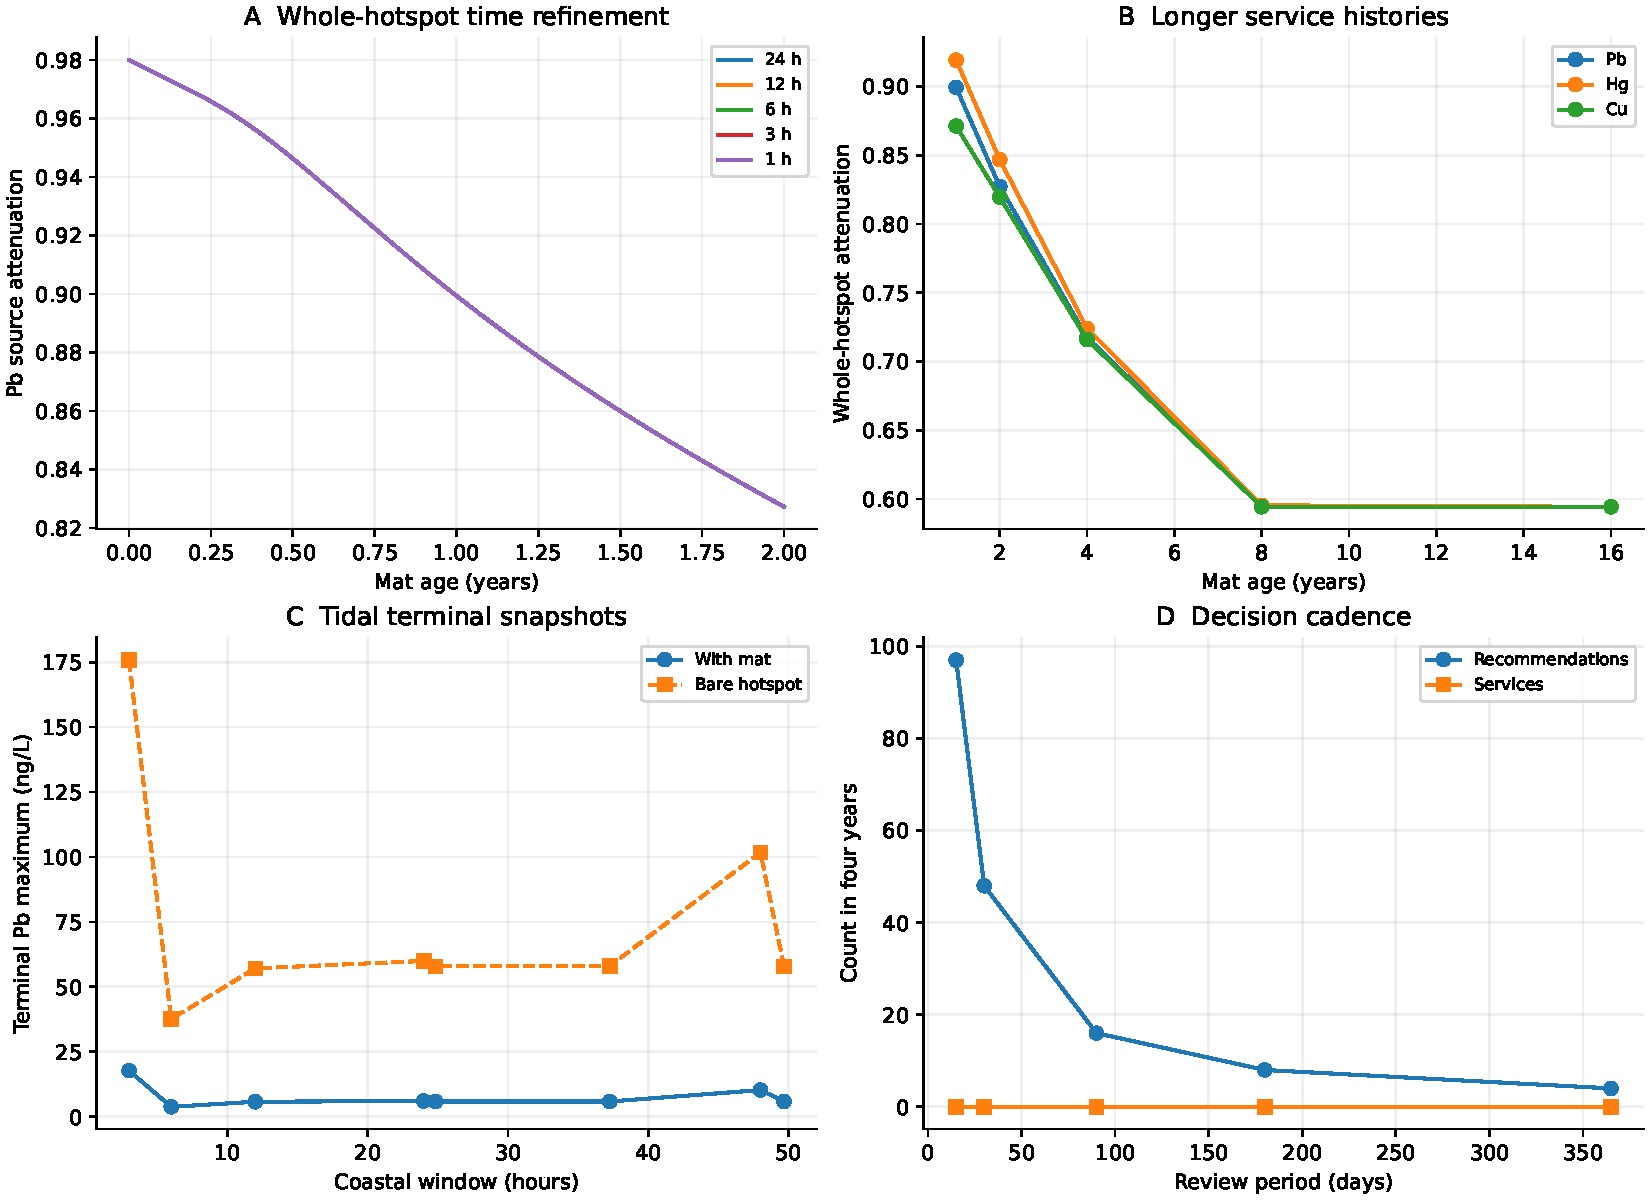
\includegraphics[width=\linewidth]{figures/timescale_audit.pdf}
\caption{Regenerated scenario studies: A, two-year whole-hotspot attenuation under time refinement; B, longer exact-age histories; C, terminal coastal maxima at different window lengths and tidal phases; D, recommendations and accepted services at different review cadences. Lines join computed samples without smoothing; the coarse horizon samples are not continuous observations.}\label{fig:timescale-audit}\end{figure}


\subsection{Coastal discretisation sensitivity}
\label{sec:coastal_refinement}

The coastal audit holds the $600\times400$~m physical domain, one-year mat
state, initial concentration, forcing phase, fixed source and 24-hour window
constant. Time steps of 600, 300 and 150~s use a 10-m grid; grids of 20, 10
and 5~m use a 150-s step. The hotspot and straight land edges align with all
three grids, avoiding a change in prescribed footprint area. The same FiPy
transport implementation is used.\citep{fipy2009}


\begin{table}[htbp]\centering\small
\caption{Fixed-window coastal time-step and grid refinement. These are numerical sensitivities rather than uncertainty intervals from material variability.}\label{tab:coastal-discretisation}
\resizebox{\linewidth}{!}{\begin{tabular}{rrrrrr}\toprule
Grid (m) & Step (s) & Pb peak: mat (ng/L) & Pb peak: bare (ng/L) & Peak ratio & Pb in water (kg) \\\midrule
10 & 600 & 6.03871 & 59.9869 & 0.1006671 & 0.000972618 \\
10 & 300 & 5.90376 & 58.6464 & 0.1006671 & 0.000868248 \\
10 & 150 & 5.86022 & 58.2138 & 0.1006671 & 0.00082418 \\
20 & 150 & 5.75969 & 57.2152 & 0.1006671 & 0.000845344 \\
5 & 150 & 5.88378 & 58.4479 & 0.1006671 & 0.000818459 \\
\bottomrule\end{tabular}}\end{table}


The 600-s versus 150-s terminal with-mat Pb peak difference at 10~m is 3.046\%; the 10-m versus 5-m difference at 150~s is -0.400\%. Each signed difference is expressed relative to the finer result. Coexisting temporal and spatial errors prevent these differences from being interpreted as bounds relative to an exact PDE solution. A stable source ratio or closed water ledger does not eliminate peak-concentration discretisation error.


For the remaining Pb inventory in the water, the corresponding differences are 18.010\% under time refinement and 0.699\% under grid refinement. The larger temporal sensitivity of this integrated field quantity further limits claims of coastal numerical accuracy based on a terminal peak alone.


\begin{figure}[htbp]\centering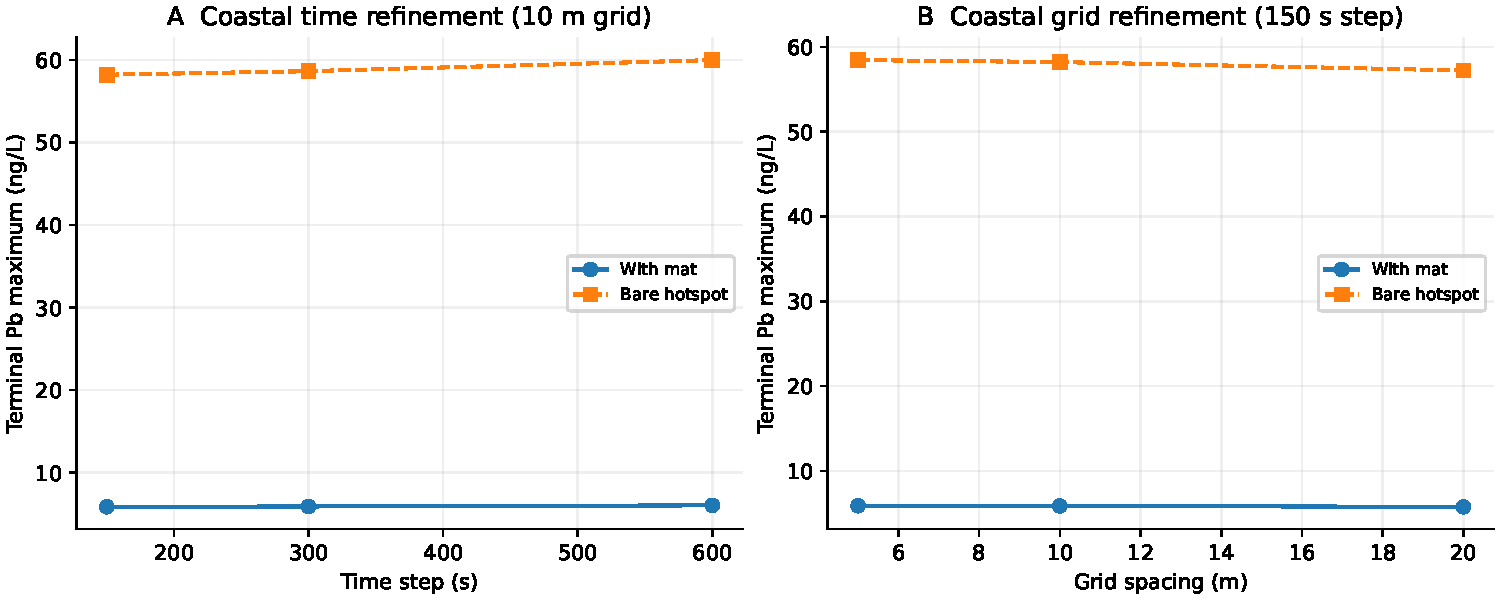
\includegraphics[width=\linewidth]{figures/coastal_discretisation_audit.pdf}
\caption{Coastal numerical sensitivity at a fixed one-year mat state and fixed 24-hour tidal window. Left: time-step refinement on the 10-m grid; right: grid refinement at 150 s. The relative with/bare source response may be more stable than either absolute terminal maximum.}\label{fig:coastal-discretisation-audit}\end{figure}

